\subsubsection{Overview}

The proper PCB layout of the driver board is just as essential as that of the power board. To keep the price of the PCBs down, both the power and the driver board has to be kept under $100mm x 100mm$. The layer number of the boards is also a pricey concern. Read more on PCB selection in Section \ref{PCB_selection}. The driver board was designed on 2-layer FR4 1 oz. material. \\

The power board was first laid out to get a precise and optimal placement of the critical components, power rails, outputs and interboard connectors. After that came defining the contour of the driver board, precise placement of interboard connectors and crude placement of components. It is vital for all signals to have their firm ground plane under them to act as reference. That is why the bottom side of the driver board was partitioned according to the components on the top side to have their respective ground planes. The surface of the cooper fills were reduced as much as possible to counter capacitive noise propagation. Supply-ground decoupling capacitors were placed as close to their supported components as possible. 0805 and 1206 size code footprints were placed to have more possibilities for modification or rework if need be. A coutout over the power rails provides space for the electrolitic capacitors attached to the bus bar. For approximate mechanical construction, see Figure \ref{fig:mech_persp} and Figure \ref{fig:mech_top}.

\begin{figure}[H]
	\centering
	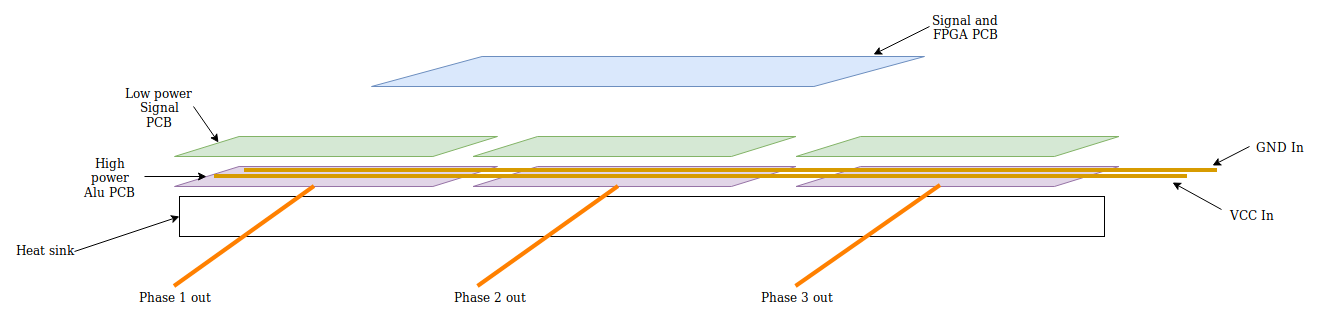
\includegraphics[width=1\textwidth]{pictures/hardware/Power_Board/mechanical_persp_new.png}
	\caption{Perspective view of mechanical construction}
	\label{fig:mech_persp}
\end{figure}

\begin{figure}[H]
	\centering
	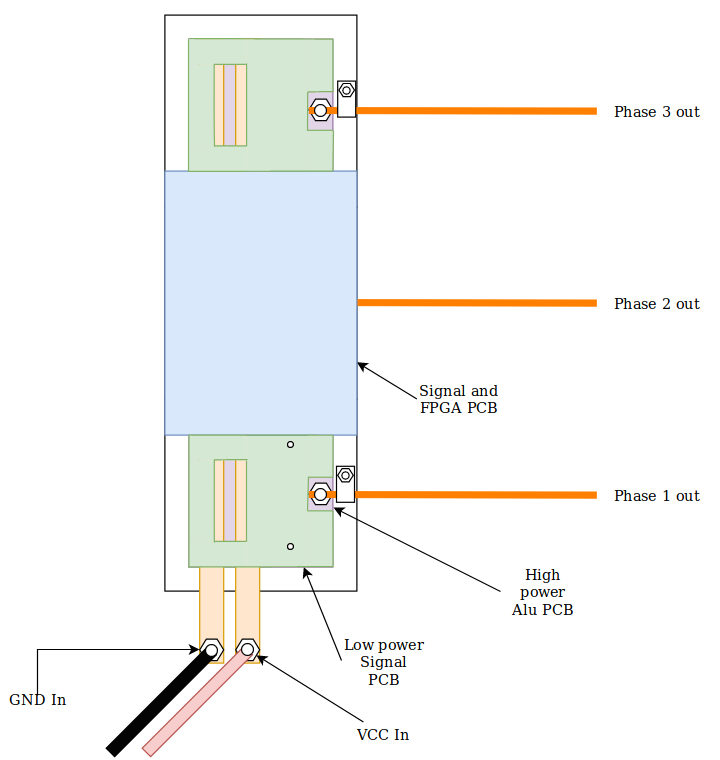
\includegraphics[width=1\textwidth]{pictures/hardware/Power_Board/mechanical_top_new.png}
	\caption{Top view of mechanical construction}
	\label{fig:mech_top}
\end{figure}



\subsubsection{Power board}

Individual PCBs of $100mm x 65mm$ were chosen for each phase. This way they would be within the general size constraints and fit the $100mm x 200mm$ heatsink that we had available. The three boards are interconnected with the power rail busbars. They have holes in them to provide a fixture point before assembly. Only the top side of the alu PCB has a copper layer. This is partitioned into 3 regions. Te first is the battery positive VCC, it is connected to the drain of the high-side MOSFETs. The common region is the output, it gives place to the high-current screw terminal. The source of the low-side FETs is connected to the battery negative GND. To provide the best supply-ground capacitive decoupling and keep the circuit highlighted in \ref{fig:cap_circ} as short as possible, capacitors are placed along the border of the VCC and GND planes. Electrolitic capacitors sit attached to the busbars. It is important to have as high capacitance as possible while keeping the ESR (Equivalent Series Resistance) and stray inductance to a minimum. This is why UVZ2A471\cite{elco} was chosen. Its small form factor provides all the aforementioned advantages. The MOSFETs are as close to each other as possible. This is limited by the presence of the interboard connector conducting the gate current. Screw holes are also present to help press the PCBA against the heatsink.

\begin{figure}[H]
	\centering
	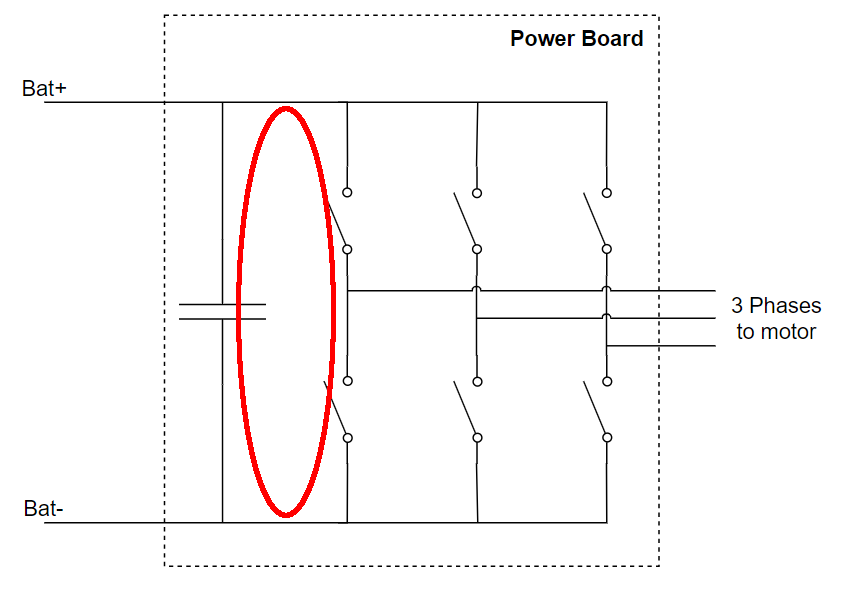
\includegraphics[width=1\textwidth]{pictures/hardware/Power_Board/Sketch_of_powerBoard_circulating.PNG}
	\caption{Perspective view of mechanical construction}
	\label{fig:cap_circ}
\end{figure}

\subsubsection{Driver board}


